\chapter{TGC~システム}
\thispagestyle{empty}
\label{chap:4}
TGC~(Thin~Gap~Chamber)~検出器~\cite{TR:04}は~MWPC~であり、wire~と~strip~が互いに交差して配置されているため二次元読み出しを可能にしたトリガー用前後方ミューオン検出器である。本章では~TGC~検出器の詳細および信号読み出しのための各エレクトロニクスについて記す。
\section{TGC~の動作原理}
TGC~は、動作ガスとして~$\rm{CO_2}$/n-Pentane(55:45)を使用している。wire~には通常~2.8~keV~の高電圧が印加されている。ガス中を荷電粒子が通過すると、その経路にあるガス分子が電離される。電離された一次電子は陽極側にドリフトしながら印加電場によって加速され、ガス分子の電離エネルギーを超えると二次電子を生成する。以上のような電子生成を繰り返すことでカスケード型の電子雪崩を生成する。電子とイオン雲はそれぞれドリフトによって互いに離れ、電子雲は~wire~を取り囲み、イオン雲はさらに周りを取り囲むように~wire~の半径方向に拡散してゆく。TGC~検出器は以上の過程でできた電子雪崩をシグナルとして~wire~から読み取る。同時に~cathode~面では、塗布された高抵抗のカーボン面に電荷が誘起され、外側の~strip~にも同様に電荷が誘起されることで信号として読み出される。

anode~wire~には直径~50~$\mu\rm{m}$~の金メッキタングステンを使用しており、wire~間隔を~1.8~mm~と小さく設計することで時間応答を向上させている。cathode~にはエポキシガラス板の片面に~1~$\rm{M}\Omega/\rm{cm}^2$~のカーボンを
塗布したものを使用している。エポキシガラスの反対側には、銅の~strip~が~wire~と直行するように配置されている。strip~間隔は、15~-~53~mm~で構成されている。ガスギャップおよび~wire~間隔が小さいことで検出器の時間応答性を向上させている。

また電子雪崩によって生じた励起分子やイオン再結合により発生する紫外線は、cathode~面やガスに衝突して発生する二次電子によって放電を起こす可能性がある。したがって紫外線を吸収する効果(クエンチ効果)のある~n-Pentane~を封入している。
\figref{fig:tgc2d}に~TGC~の信号読み出しの概念図、\figref{fig:TGCpri}に~TGC~検出器の詳細な構成を示した。

\begin{figure}[H]
        \centering   
        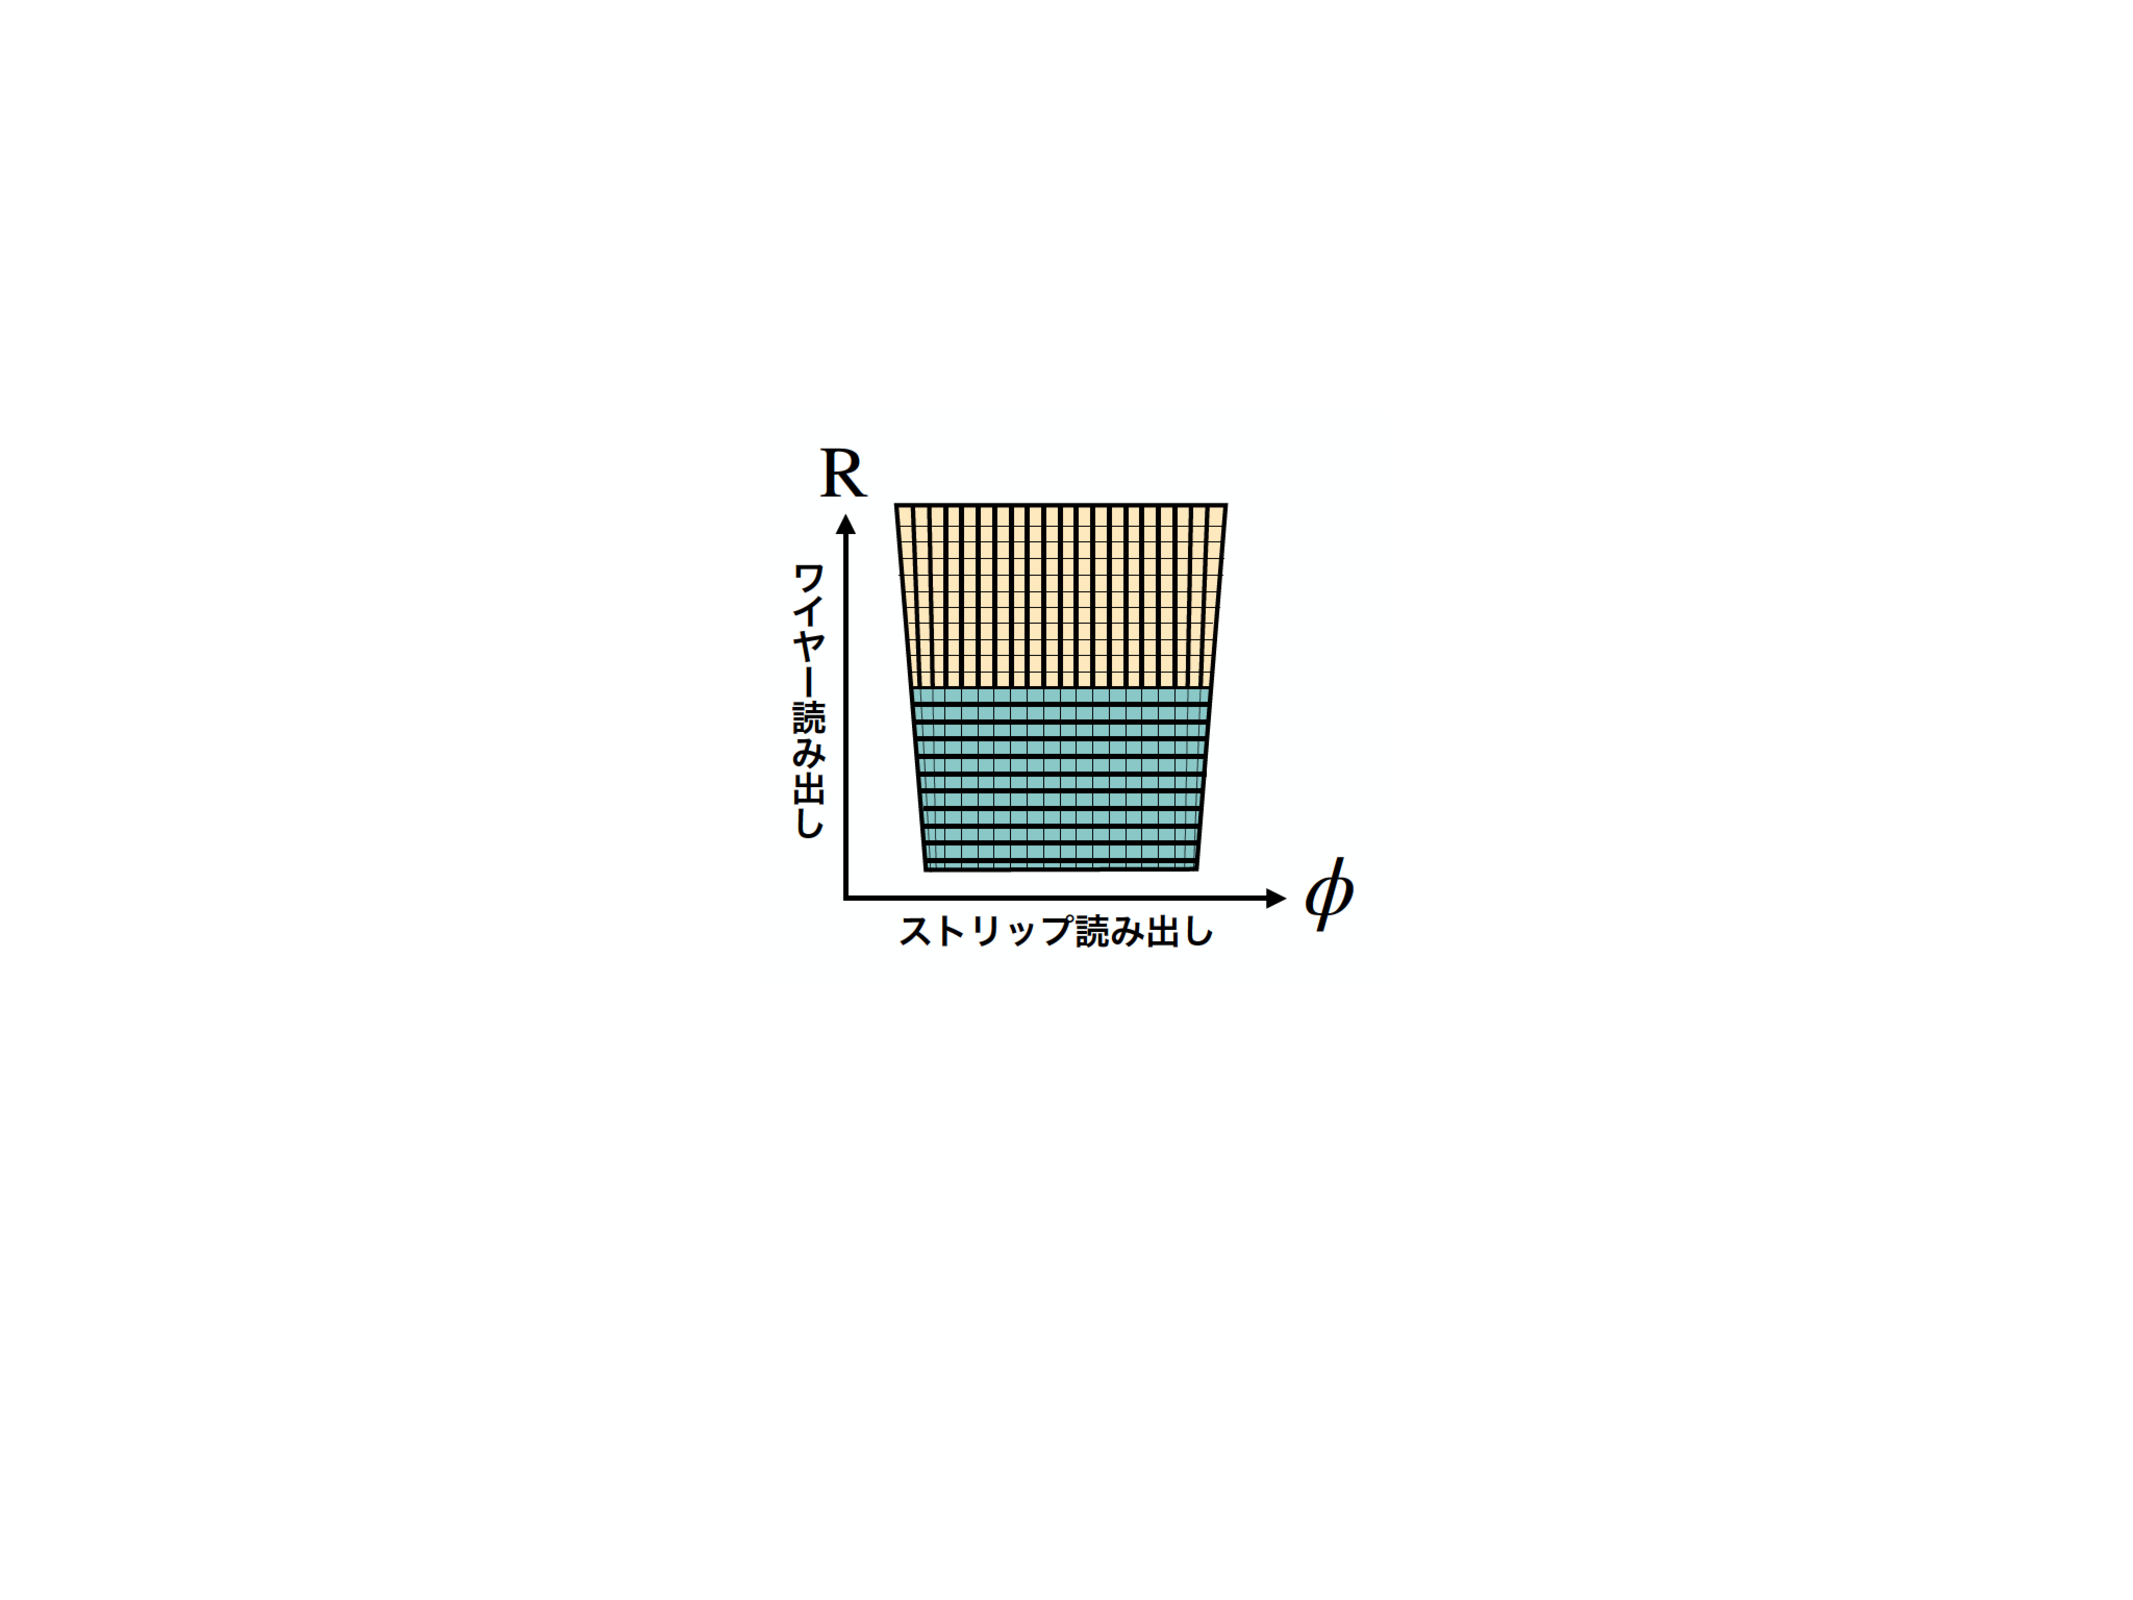
\includegraphics[width=0.6\textwidth,page=1]{img/pdf/tgc2d.pdf}
        \caption[TGC~二次元信号読み出しの概念図]{TGC~二次元信号読み出しの概念図。wire~で~$R$~方向を測定し、strip~で~$\phi$~方向を測定する。}\label{fig:tgc2d}
\end{figure}

\begin{figure}[H]
        \centering   
        \includegraphics[width=\textwidth,page=10]{img/pdf/ATLAS.pdf}
        \caption[TGC~検出器の~triplet~および~doublet~における断面図]{TGC~検出器の~triplet~および~doublet~における断面図~\cite{TR:01}。}\label{fig:TGCpri}
\end{figure}

\section{TGC~検出器}
ATLAS~実験で使用されている~TGC~検出器はエンドキャップ部に設置されたミューオントリガー用検出器であり、総数として約~3700~枚で、全チャンネル数は~R~方向に約~22~万(wire)、$\phi$方向に約~10~万(strip)という数で構成されている。\figref{fig:tgc00}に~TGC~検出器の全体写真を示した。

TGC~検出器は大きくエンドキャップマグネットの外側に位置する~Big~Wheel~と内側に位置する~Small~Wheel~に分けられる。
Big~Wheel~は、M1(3~層)、M2(2~層)、M3(2~層)の計~7~層で構成されており、トリガー判定には主に以上の7層が利用されている。Small~Wheel~は、EIFI(2~層)で構成されており、フェイクミューオンの誤ったトリガーの削減等の役割を持つ。以下では、TGC~検出器それぞれの役割や配置等の詳細について述べる。

\begin{figure}[H]
    \centering   
    \includegraphics[width=0.75\textwidth,page=15]{img/pdf/ATLAS.pdf}
    \caption[TGC 検出器のビーム軸方向から見た全体写真]{TGC~検出器のビーム軸方向から見た全体写真~\cite{TR:01}。写真は~BW~の~M1~ステーション。}\label{fig:tgc00}
\end{figure}

\subsection{Big Wheel}
M1、M2~および~M3は~Big~Wheel~と呼ばれる。\figref{fig:tgcBW}に~TGC~M1~の配置図を示した。
Big~Wheel~は~$1.05~<~|\eta|~<~2.7$~の領域をカバーし、$|\eta|~<~1.9$~の領域をエンドキャップ、$|\eta|~>~1.9$~の領域をフォワードと呼ぶ。

Big~Wheel~は~TGC~を~$\phi$~方向に~12~等分した~1/12~円を一つの大きな単位としており、これを~1/12~セクターと呼ぶ。データ処理などはこの単位で行われ、。初段トリガーに関連する部分では、1/12~セクターはさらに~$\phi$~方向にエンドキャップで~4~等分、フォワードで~2~等分され、それぞれをトリガーセクターと呼ぶ。さらにトリガーセクターはエンドキャップ領域では~$\eta$~方向~37~分割、$\phi$~方向に4分割、フォワード領域では~$\eta$~方向に16分割、$\phi$~方向に4分割され、それぞれをサブセクターと呼ぶ。サブセクターは~8~ワイヤグループと~8~ストリップに対応しており、トリガー処理の最小単位となっている。運動量の概算に利用される~RoI~はサブセクターにおいて番号付けされる。\figref{fig:tgcsector}にセクターと~RoI~の番号付けの詳細を示した。

\begin{figure}[H]
		\begin{minipage}{0.49\hsize}
		\centering
        \includegraphics[width=\textwidth,page=2]{img/pdf/TGC.pdf}
        \end{minipage}
        \begin{minipage}{0.49\hsize}
        \centering
        \includegraphics[width=\textwidth,page=3]{img/pdf/TGC.pdf}
        \end{minipage}
        \caption[TGC 検出器~Big~Wheel~M1~ステーションの配置図]{TGC~検出器~Big~Wheel~M1~ステーションの配置図~\cite{TR:02}。$\phi$~方向に対して、エンドキャップでは~48~分割、フォワードでは~24~分割されている。A-Side(左)、C-Side(右)。}
        \label{fig:tgcBW}
\end{figure}

\begin{figure}[H]
        \centering   
        \includegraphics[width=0.8\textwidth,page=8]{img/pdf/TGC.pdf}
        \caption[トリガーセクターと~RoI~の番号付け]{相互作用頂点から見た~A-Side~のトリガーセクターと~RoI~の番号付け~\cite{TR:02}。$\phi,~\eta$~方向に~RoI~の番号が振り分けられている。}
        \label{fig:tgcsector}
\end{figure}

\subsection{Small~Wheel}
Small~Wheel~は~EIFI~チェンバーで構成されており、$1.05~<|\eta|~<~1.9$~の領域をカバーしている。\figref{fig:tgcSW}に~TGC~EIFI~の配置図を示した。Big~Wheel~とは異なる特徴的な配置となっている。特に~EI~チェンバーが特徴的で所々に隙間が存在する構成になっている。これはバレル部分のトロイドマグネットの配置の影響によるものである。EI~チェンバーがあるセクターをラージセクター、ないセクターをスモールセクターと呼ぶ。

\begin{figure}[H]
        \centering   
        \includegraphics[width=0.9\textwidth,page=4]{img/pdf/TGC.pdf}
        \caption[TGC 検出器~Small~Wheel~EIFI~ステーションの配置図]{TGC~検出器~Small~Wheel~EIFI~ステーションの配置図。内側が~FI~T10~チェンバー、外側が~EI~T11~チェンバー。EI~は支持構造との干渉を避けるため~8~箇所の隙間が存在する。C-Side(左)、A-Side(右)~\cite{TR:02}}
        \label{fig:tgcSW}
\end{figure}

\subsection{TGC~の~ネーミング~と~ナンバリング}
TGC~検出器は膨大な数が設置されている。TGC~を効率よく共通の認識で区分するためにネーミングとナンバリングが施されている。以下では~TGC~の共通区分の方法について記す。
\subsubsection{TGC~のネーミング}
生産ラインから出てくる~TGC~検出器一つを示す基本単位を「ユニット」とする。このユニットには、外形寸法によって名前が付けられており、T01~から~T11のメジャータイプがある。wire~の~ASD~ボックス(詳細は\subsubsecref{subsubsec:ASD}で述べる)は、台形のどちらの側にも配置することが可能で、各ホイールには~Forward~型と~Backward~型のユニットがある。\figref{fig:tgcBF}にフロントエンドエレクトロニクスを含めた~TGC~ユニットの詳細を示す。パリティ不変性を保つために、2つのエンドキャップは互いに鏡像になっている。

strip~の場合、ガスフローの接続の関係でタイプT01~T05、T07、T10では台形の辺の長さが大きい部分(アウター)から、タイプT06、T08、T09、T11では辺の長さが小さい部分(インナー)から読み出されることになる。この違いは、ネーミングには反映されていない。

あるメジャータイプのユニットは、M1、M2、M3、EIFI~の~4~つのステーションで区分することができる。1~は~M1(トリプレット)、2~と~3~は~M2~と~M3(ダブレット)、4~は~EIFI(ダブレット)である。メジャータイプはさらにマイナータイプへと区別され、I(インテグラル、またはレギュラー)、H(アライメント通路のスペースを確保するために空洞化)、S(スペシャルまたはショートチャンバー)に分類される。I~と~H~に関しては外形寸法に違いはない。しかし~S~に関しては外形寸法や~ASD~ボックスの配置にも違いがある。S~に分類される場合があるのは、EIFI~のみでありこの違いは本研究においても重要であるのでここで言及しておく。\tbref{tb:unit1}、\tbref{tb:unit2}にその全容をまとめる。

\begin{figure}[h]
        \centering   
        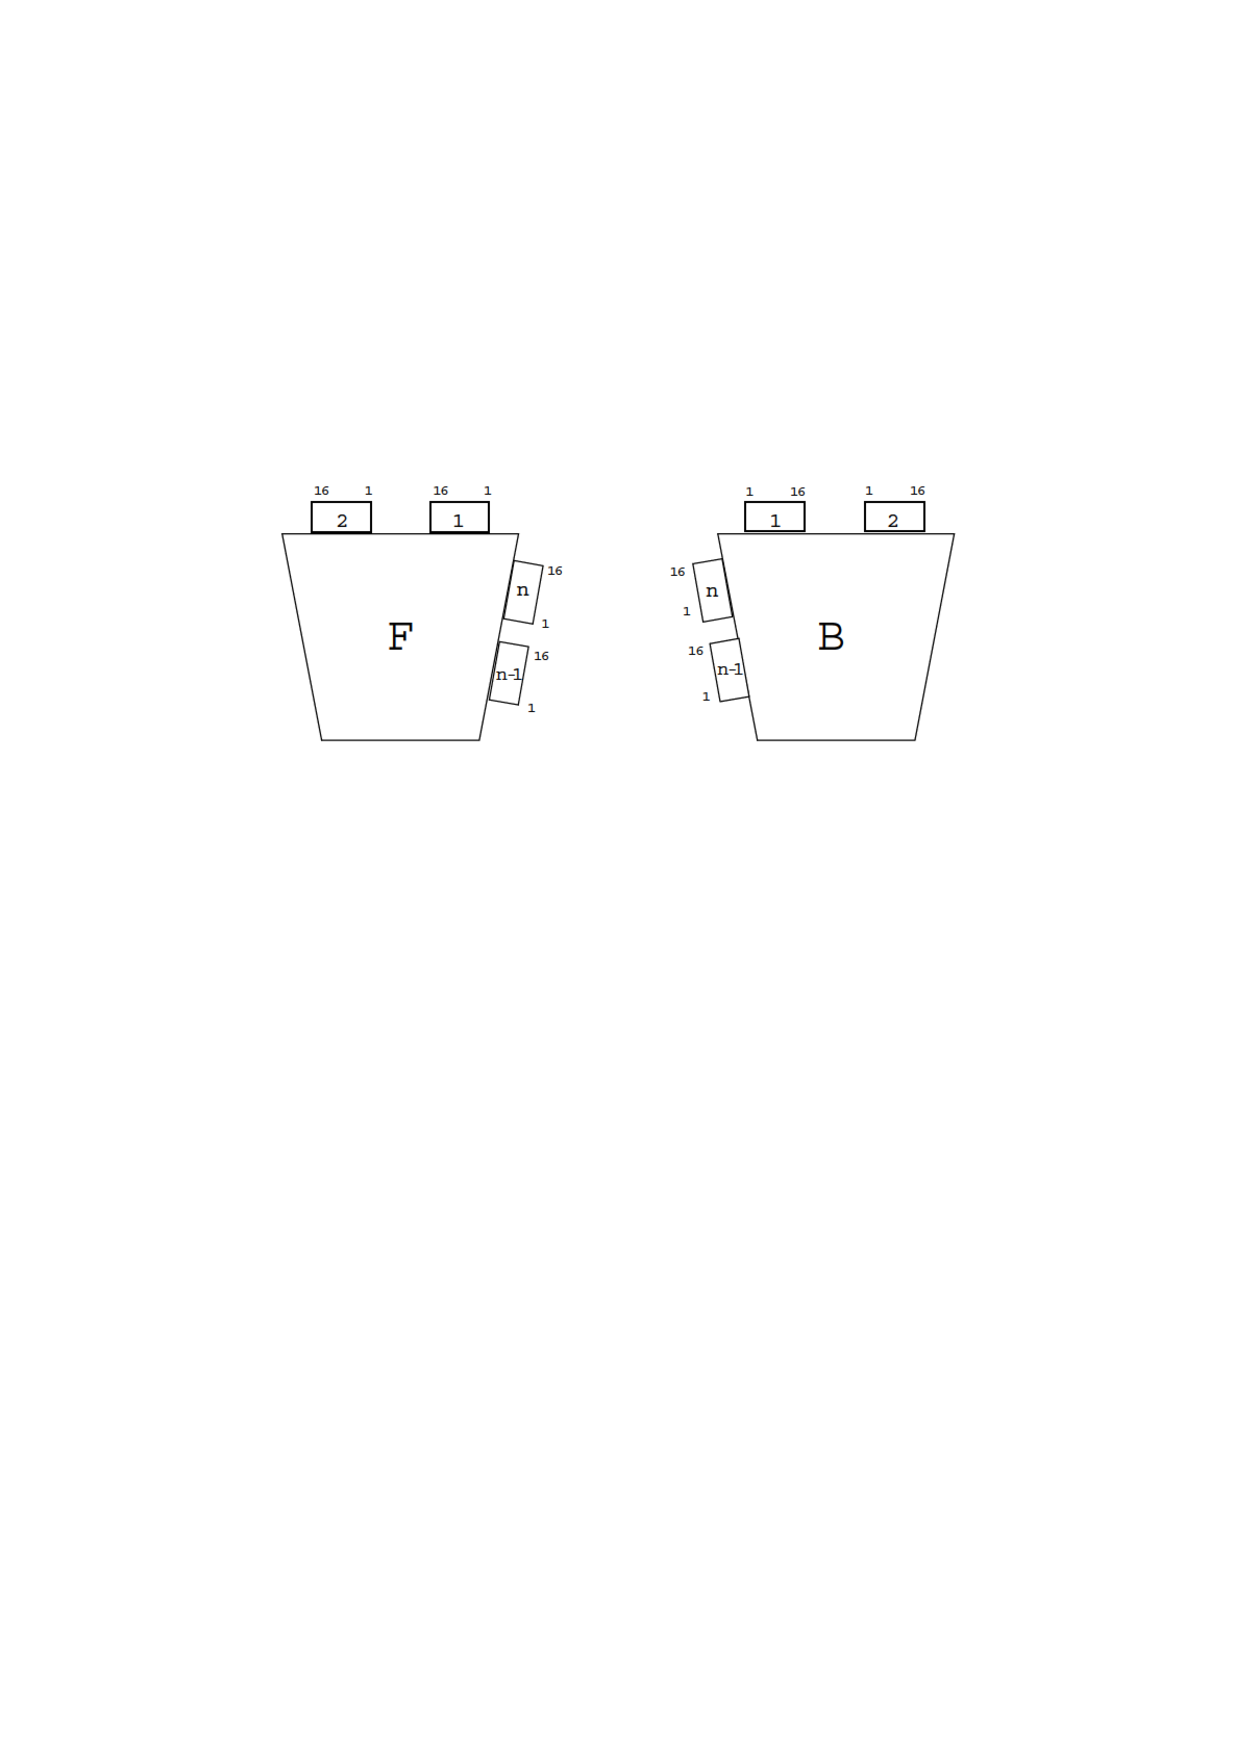
\includegraphics[width=0.8\textwidth,page=1]{img/pdf/TGC.pdf}
        \caption[フロントエンドエレクトロニクス、ASD~および~ボードを搭載したフォワードユニットとバックワードユニット]{フロントエンドエレクトロニクス、ASD~および~ボードを搭載したフォワードユニットとバックワードユニットを初期相互作用点から見た様子~\cite{TR:02}。}
        \label{fig:tgcBF}
\end{figure}

\begin{table}[tb]
	\centering
	\begin{tabular}{c|llll}\hline
		 ユニット & メジャータイプ & B/F & ステーション & マイナータイプ \\ \hline
		 &01..11& B = Backward & 1 = M1(triplet)& I = Integral \\
		 && F = Forward  & 2 = M2(doublet)& H = Hollowed \\
		 &&              & 3 = M3(doublet)& S = Short    \\
		 &&              & 4 = EIFI(doublet)& \\
	\end{tabular}
	\caption[TGC~におけるユニットの型名命名法]{TGC~におけるユニットの型名命名法~\cite{TR:02}。}
	\label{tb:unit1}
\end{table}

\begin{table}[tb]
	\centering
	\begin{tabular}{c|l}\hline
		 メジャータイプ & \multicolumn{1}{c}{ユニット(数)}\\ \hline
		~T01~&~B1H(8),~B1I(16),~F1H(8),~F1I(16)~\\
		~T02~&~B2H(8),~B2I(16),~B3H(8),~B3I(16)~\\
		     &~F2H(8),~F2I(16),~F3H(8),~F3I(16)~\\
		~T03~&~B1I(48),~F1I(48)~\\
        ~T04~&~B2I(48),~F2I(48)~\\
		~T05~&~B3I(48),~F3I(48)~\\
		~T06~&~B1H(8),~B1I(40),~B2H(8),~B2I(40)~\\
		     &~B3H(8),~B3I(40),~F1H(8),~F1I(40)~\\       
		     &~F2H(8),~F2I(40),~F3H(8),~F3I(40)~\\
		~T07~&~B1I(48),~B2I(48),~B3I(48)~\\
		     &~F1I(48),~F2I(48),~F3I(48)~\\
		~T08~&~B1I(48),~B2I(48),~B3I(48)~\\
		     &~F1I(48),~F2I(48),~F3I(48)~\\
		~T09~&~B2I(48),~B3I(48),~F2I(48),~F3I(48)~\\
		~T10~&~B4I(16),~B4S(8),~F4I(16),~F4S(8)~\\
		~T11~&~B4I(20),~B4S(2),~F4I(20),~F4S(2)~\\
	\end{tabular}
	\caption[TGC~におけるユニット名一覧とその数の内訳]{TGC~におけるユニット名一覧とその数の内訳~\cite{TR:02}。ユニットにおける~F,~B~はそれぞれForward,~Backward~を表す。1~から~4~の数字はステーションを表す。I,~H,~S~はそれぞれ~Integral,~Hollowed,~Short~を表す。}
    \label{tb:unit2}
\end{table}

\subsubsection{チャンネルナンバリング}
doublet~の場合、wire~と~strip~の両方が、フロントエンドエレクトロニクスによって完全に読み出される。triplet~3~層の内、中央のチェンバーでは、wire~のみが読み出される。
コネクタのチャンネル番号と整合性をとるため、以下のような規則にしたがって~ASD~ボードを通してチェンバーから~1~n~までのチャンネル番号がつけられている。\figref{fig:tgcT}に~TGC~ユニットにおける構成およびチャンネルの番号の詳細について示す。
\begin{itemize}
\item wire: \\
チャンネル~1~は、ビームに最も近い(つまり台形の小さな底面に近い)。
\item strip: \\
チャンネル~1~は、ワイヤーの~ASD~ボックスの側面に最も近い。したがって、初期相互作用点に座って検出器のホイールを観察している観察者にとって、ストリップの読み出しは、後方検出器の場合は時計回りに、前方検出器の場合は反時計回りに進む。
\end{itemize}

\begin{figure}[H]
		\begin{minipage}{0.49\hsize}
		\centering
        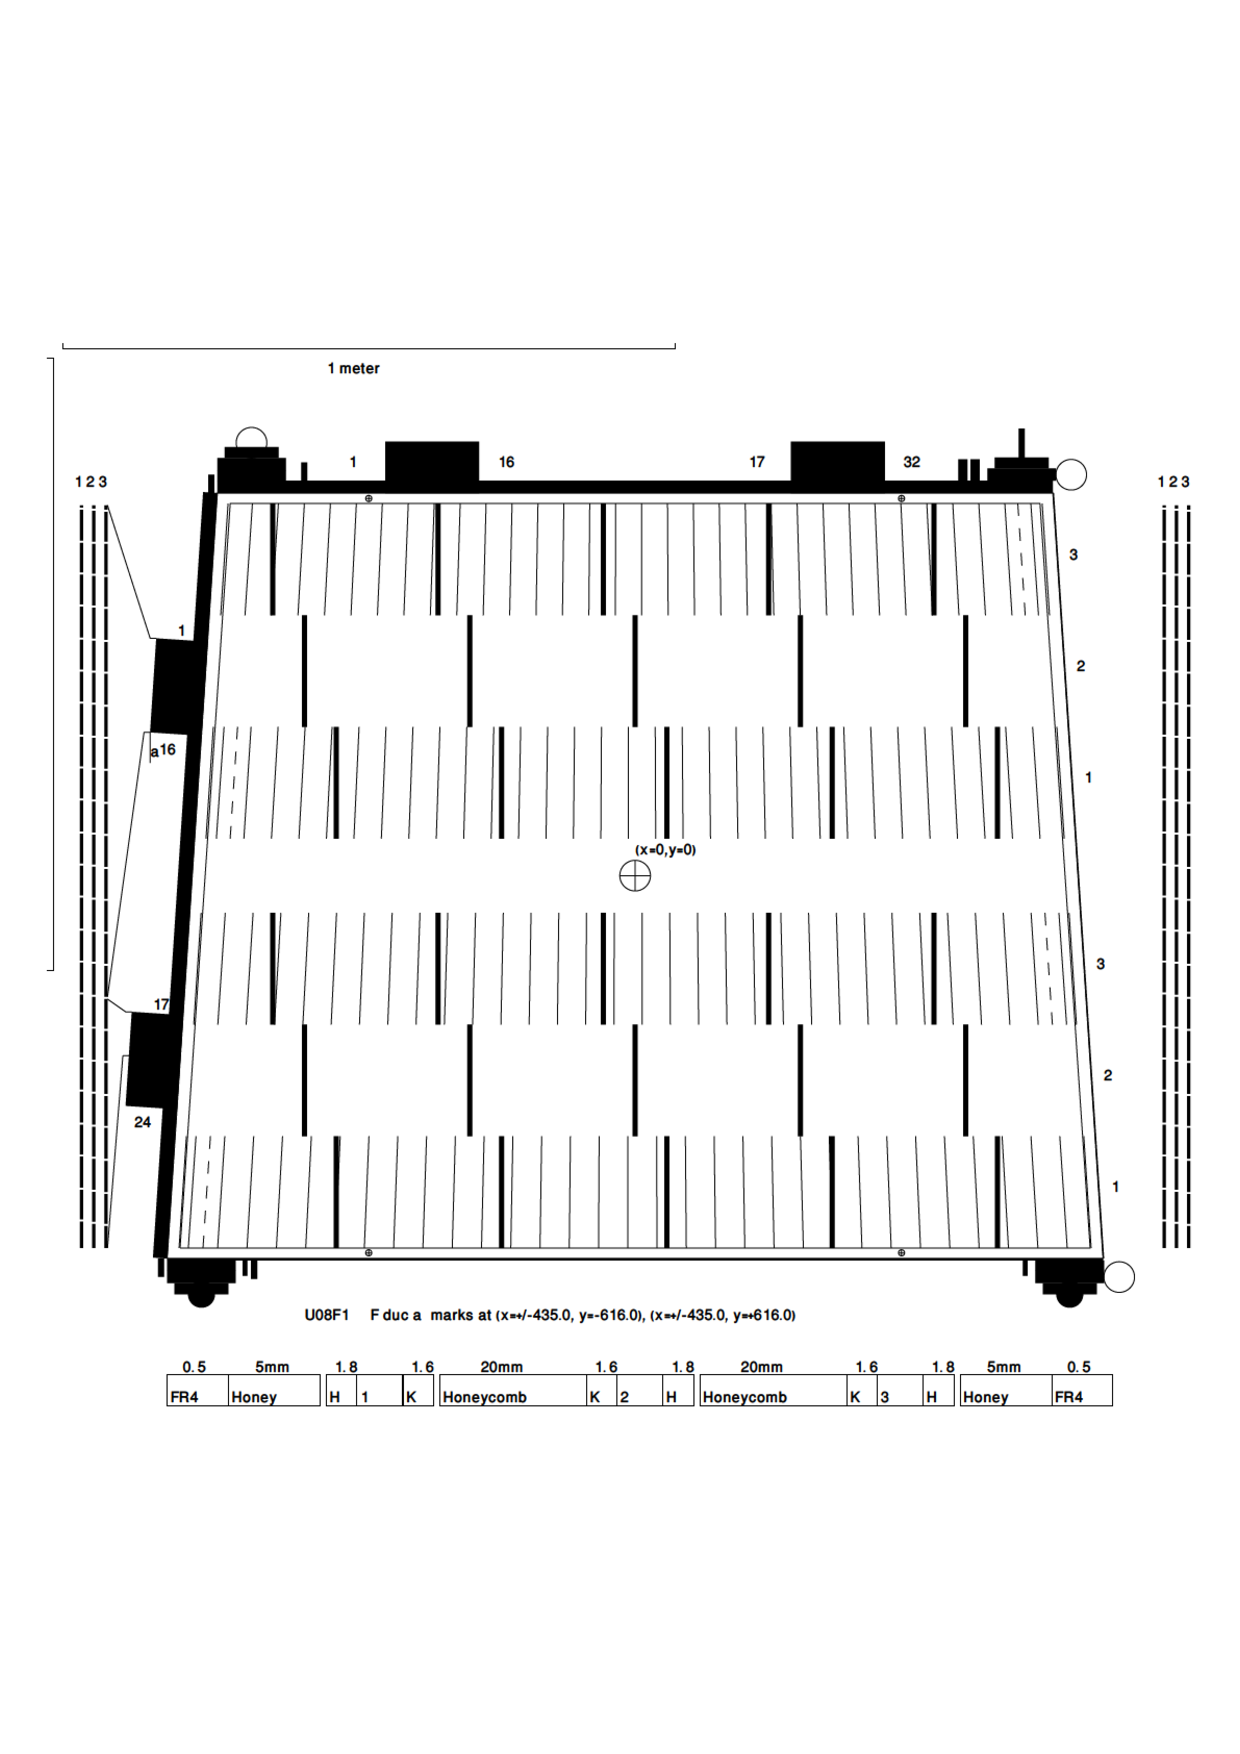
\includegraphics[width=0.9\textwidth]{img/pdf/u08f1i.pdf}
        \subcaption{}
        \end{minipage}
        \begin{minipage}{0.49\hsize}
        \centering
        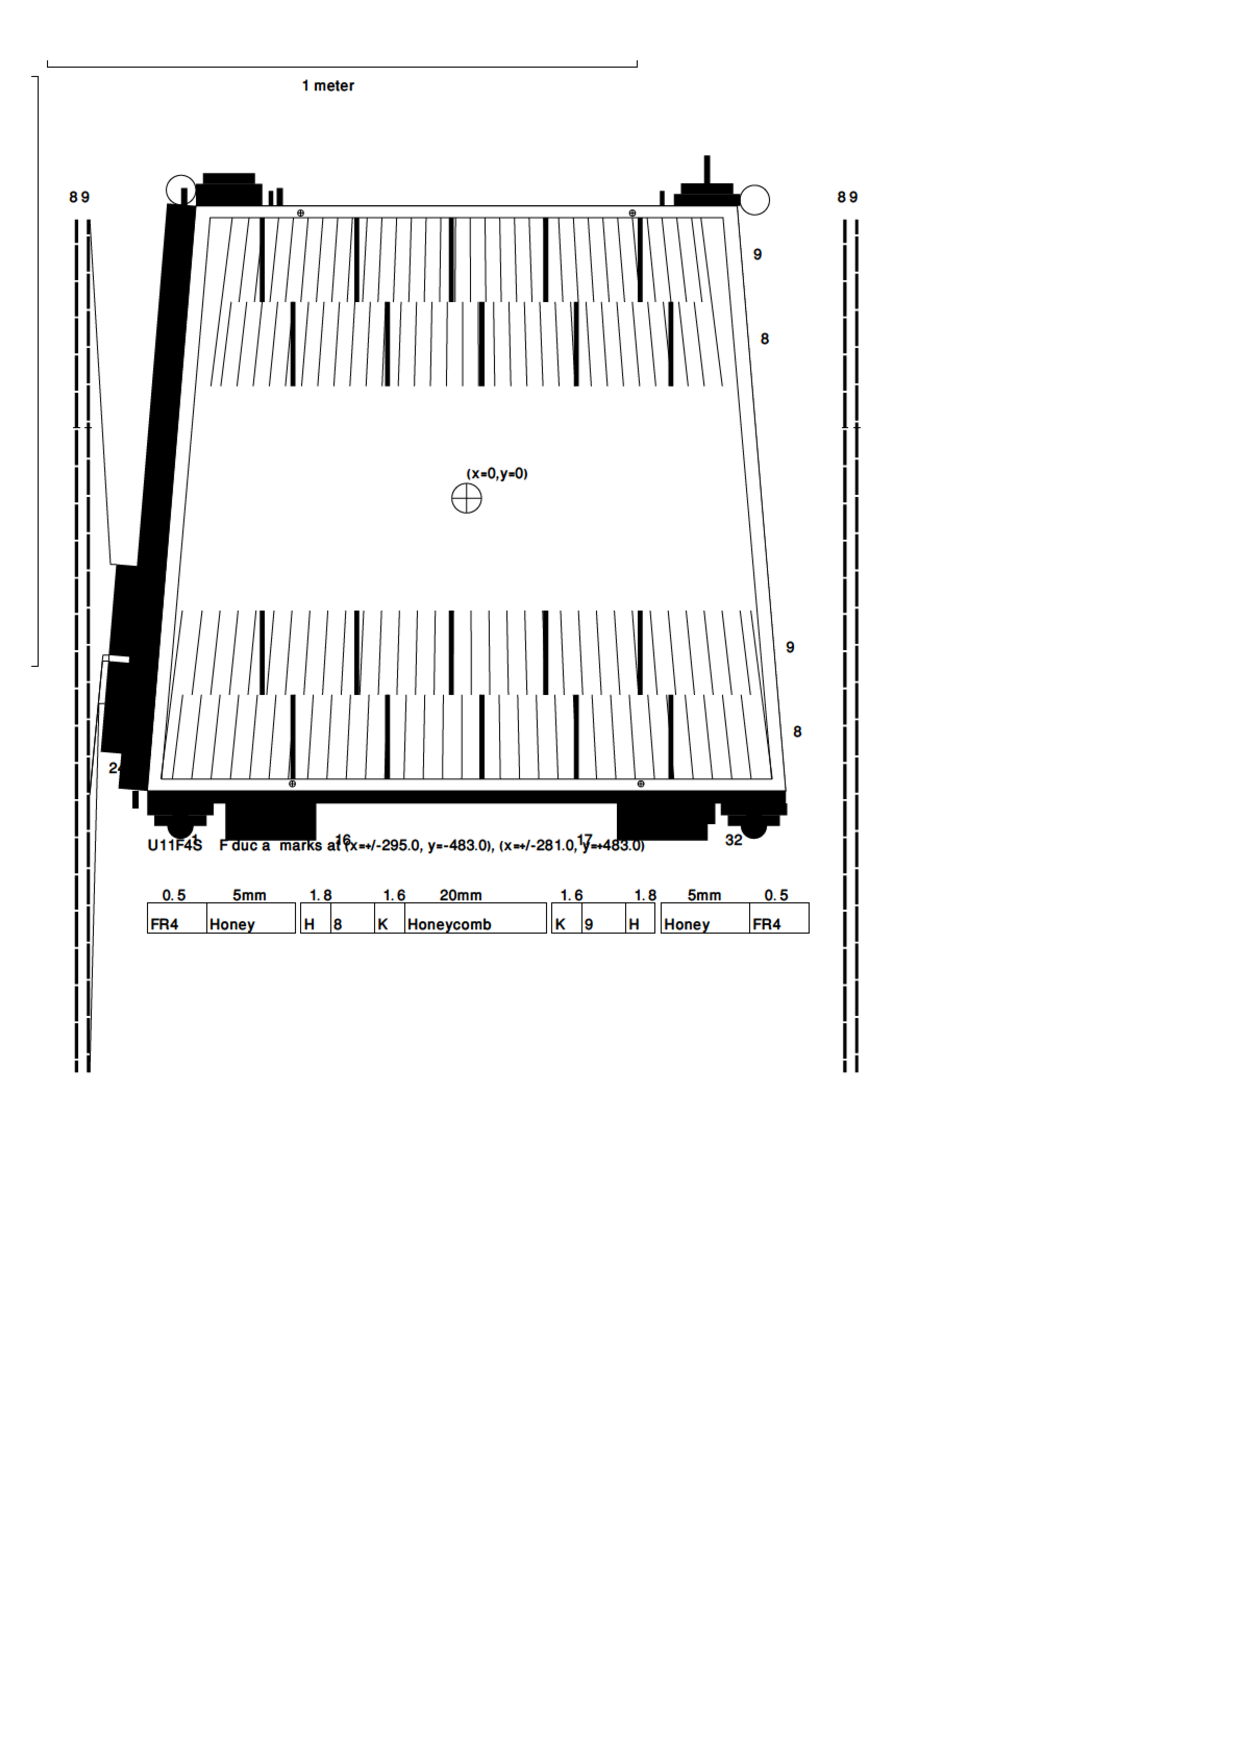
\includegraphics[width=0.9\textwidth]{img/pdf/u11f4s.pdf}
        \subcaption{}
        \end{minipage}
        \caption[TGC~検出器の構成の一例]{TGC~検出器の構成の一例~\cite{URL:04}。図の縦方向に~strip~センサー、横方向に~wire~センサーが設置されている。また~wire~および~strip~方向にそれぞれ~2~つの~ASD~が設置されている。チャンネルナンバリングについても記載している。(a)~T08~チェンバーにおける~F1I~ユニット。(b)~T11~チェンバーにおける~F4S~ユニット。}
        \label{fig:tgcT}
\end{figure}

\subsubsection{TGC~のジオメトリの概要}
TGC~システムは、互いに鏡像となる~A~と~C~の~2~つの側面で構成されている。A~は~$+z$~軸側、C~は~$-z$軸~側である。トンネルの傾斜($1.23\%$)のため、C~は~A~より約~30~cm~上に位置している。これは標準的な~ATLAS~の座標系である。
TGC~セグメンテーションは以下の通りである。
\begin{itemize}
    \item $\eta$ には、2 つの完全に独立した領域が存在する。フォワード ($1.6<|\eta|<2.0$) と エンドキャップ ($1.0<|\eta|<1.6$)。
    \item フォワード領域の $\phi$ 分割は 24(検出器角度分割 = 15 度)。
    \item エンドキャップ領域の最小の $\phi$ 分割は 48(検出器角度分割 = 7.5 度)。
    \item エンドキャップ領域のユニットは、半径方向に 4 台(M1)および 5 台(M2、M3)の「モジュール」(ラダー)に組み立てられる。
    \item エンドキャップ領域では、2つのモジュールはさらに2×4または2×5の「セット」にグループ化される。このグループのうち、一方は~Backward ユニット、もう一方は~Forward ユニットで構成される。フォワード領域では、各ユニットはモジュールであると同時にセットでもある。
    \item 1つのフォワード検出器と1つのエンドキャップ・セットのユニットのアセンブリは、それ自体がセットと呼ばれ、基本的な物理的アセンブリとなる。
\end{itemize}
\tbref{tb:tgcNaming}、\tbref{tb:4tgc}に TGC のジオメトリにおける詳細な位置の命名法をまとめる。

\begin{table}[tb]
	\centering
	\begin{tabular}{llll}\hline
	A/C & ステーション & Ei/F & $\phi$ \\ \hline
	Side & 1 = M1  & E1 = エンドキャップの最も外側 & 0..23(フォワード)\\
	& 2 = M2 & E4 or E5 = エンドキャップの最も内側 & 0..47(エンドキャップ)\\
	& 3 = M3 & F = フォワード & \\
	& 4 = EIFI &&
	\end{tabular}
	\caption{TGC の命名法}
	\label{tb:tgcNaming}
\end{table}

\begin{table}[tb]
	\centering
	\begin{tabular}{c|cccccc}\hline
	& \multicolumn{6}{|c|}{$|\eta|$ ---------------------->} \\
	ステーション & E1 & E2 & E3 & E4 & E5 & F \\ \hline
	1 = M1 & T08 & T07 & T06 & T03 & & T01 \\
	2 = M2 & T09 & T08 & T07 & T06 & T04 & T02 \\
	3 = M3 & T09 & T08 & T07 & T06 & T05 & T02 \\
	4 = EIFI & T11 &&&&& T11 \\
	\end{tabular}
	\caption{各ステーションにおけるメジャータイプの割り当て}
	\label{tb:4tgc}
\end{table}

\section{TGC~での運動量概算}
エンドキャップのミューオントリガーシステムは、BW~における~7~層の~TGC~検出器のコインシデンスを利用している。さらに~7~層の検出点の位置情報を利用した運動量の概算により、運動量のラベル付けを行ったコインシデンス情報を出力できるトリガー系となっている。\figref{fig:tgcpt}に~$p_{\rm{T}}$~の大きさによって変化する飛跡の一例を示した。

また、\figref{fig:tgcptt}は~TGC~における運動量概算の概念図である。エンドキャップ領域のミューオントリガーシステムにおける運動量の概算方法としては、全検出層が磁場の外にあり磁場中のトラックの曲率を直接測ることはできないため、代わりに~7~層の~TGC~検出器を用いて再構成した直線飛跡を用いて運動量を概算を行う。TGC~トリガー回路系は複数層のヒットコインシデンスに基づき直線飛跡を再構成し、衝突点を向いたトラックを選ぶことで、高運動量のミューオンを選別するトリガーとして機能する。この手法を~Point~Angle~Measurement~と呼ぶ。

7~層のTGC~検出器、M1、M2、M3~はそれぞれ~z~=~13~m,~z~=~14~m,~z~=~14.5~m~に位置している。TGC~は~wire~と~strip~の直交した二つの読み出しから荷電粒子の通過位置を決定する。wire~が~$\eta$~方向を測定し、strip~が~$\phi$~方向を測定する。必要十分な位置分解能を達成するためのチャンネル幅は~wire、strip~ともに~$O(1~\rm{cm})$~となっている。トリガーロジックは~M3~におけるヒットを~Pivot~として用いて~Point~Angle~Measurement~を行う。

また、エンドキャップトロイド磁石よりも衝突点に近い側に位置する~EIFI~とのコインシデンスを取ることで、衝突点から飛来したミューオンに対して選択的にトリガーを行なっている。

\begin{figure}[H]
        \centering   
        \includegraphics[width=\textwidth,page=13]{img/pdf/ATLAS.pdf}
        \caption[初段エンドキャップミューオントリガーにおけるミューオンの飛来の様子と~RoI~の詳細]{初段エンドキャップミューオントリガーにおけるミューオンの飛来の様子と~RoI~の詳細~\cite{TR:01}。左図は~TGC~検出器の断面図であり、ミューオンの~$p_{\rm{T}}$~の大きさによるふるまいの違いを示している。右図は~TGC~のトリガーセクターと~RoI~を表しており、緑の線で囲まれた部分が~1~トリガーセクターを示す。赤で囲まれた部分が~1~RoI~を表す。}
        \label{fig:tgcpt}
\end{figure}

\begin{figure}[H]
        \centering   
        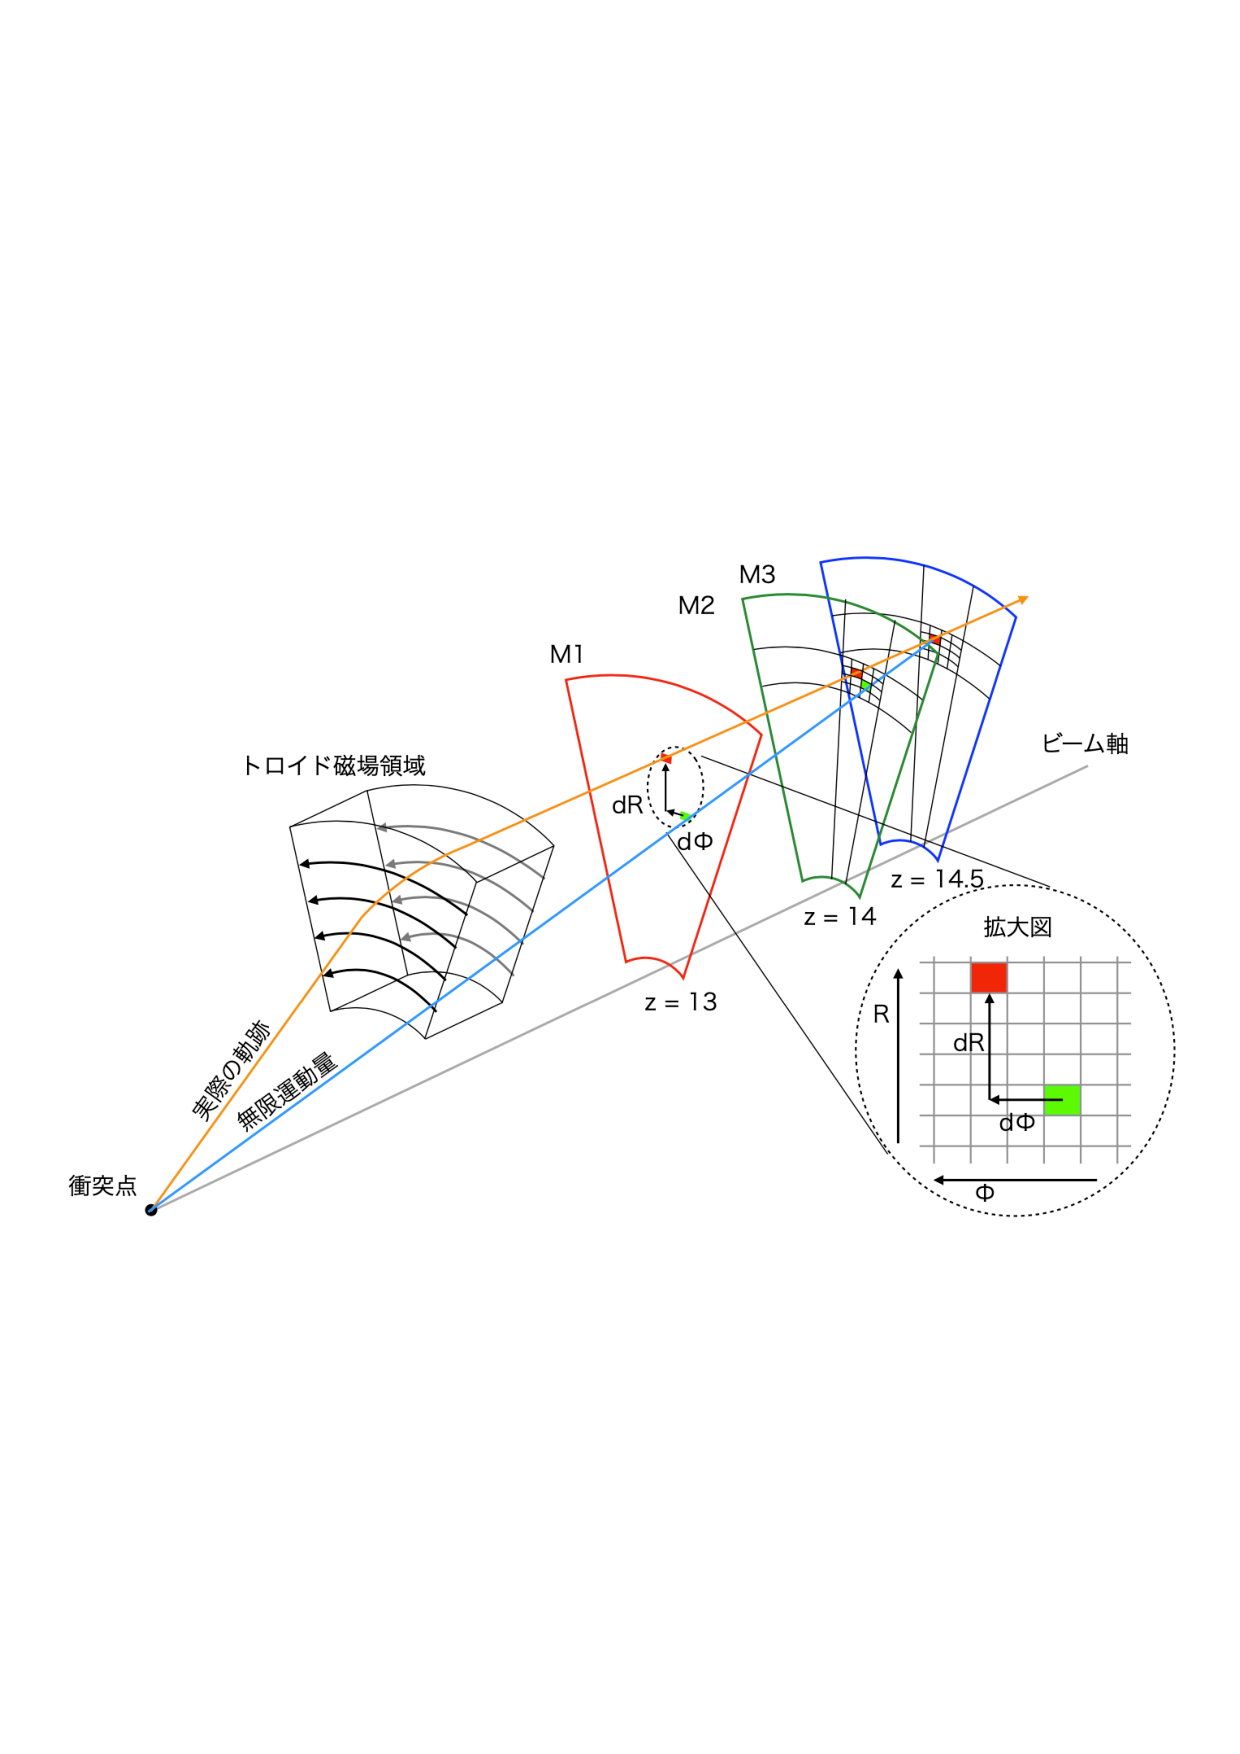
\includegraphics[width=0.9\textwidth,page=1]{img/pdf/pttgc.pdf}
        \caption[TGC~BW~におけるミューオンの運動量概算の概念図]{TGC~BW~におけるミューオンの運動量概算の概念図~\cite{MT:03}。ミューオンが残すヒット点と直線飛跡との$R,~\phi$~方向との差からミューオンの横運動量を概算する。}
        \label{fig:tgcptt}
\end{figure}

TGC~検出器は~Triplet~内、Doublet~内のローカルなコインシデンスをもちいてデータリダクションを行い、最終的に~3~ステーションコインシデンスによりトリガー判定を行う。手順は以下の通りである。
\begin{itemize}
\item ミューオンが通過し、7~層の~wire~と~6~層の~strip~にそれぞれヒットを残す。
\item ステーション内の~2~層または~3~層のコインシデンスをもちいてノイズのヒットをのぞき、かつコインシデンス結果より各ステーションにおける通過位置を$~R$,~$\phi$~で別々に求める。
\item M2、M3~の間でのコインシデンスをとって~Doublet~4~層でのトラックセグメントを求める。このとき~$dR_{23}=R_2-R_3$、$d\phi_{23}=\phi_2-\phi_3$~が運動量の指標として用いられ、小さいものだけをトラック候補として残す。
\item M2、M3~のコインシデンス結果と~M1~の間で、さらにコインシデンスをとる。M2、M3~の間のコインシデンスで行なったように、$R_{13}=R_1-R_3$~と~$d\phi_{13}=\phi_1-\phi_3$~の情報を用いてトラック候補の選別を行う。ここまでは~wire~($R$)~と~strip~($\phi$)は別々に計算される。
\item 最後に、$R~$と~$\phi$~の情報のコインシデンス情報を合わせて、RoI~を形成し、さらに~$dR$~および~$d\phi$~の情報を合わせて運動量判定を行う。この運動量判定情報および~RoI~の情報が~MUCTPI~に送られる。
\end{itemize}

\section{TGC~エレクトロニクス}
TGC~システムの電気回路系におけるデジタル電気回路の設置箇所は大きく以下の~3~つに分かれる。
\begin{itemize}
    \item PS Board: \\
    Patch~Panel~ASIC~(PP)~と~Slave~Board~ASIC~(SLB)~が設置されている。
    \item ミニラック:\\
    読み出し用のモジュールである~Star~Switch~(SSW)~と、M1、M2、M3~のコインシデンスのための~High~PT~(HPT)~が搭載されている。
    \item USA15: \\
    USA15~に読み出しのための~Readout~Driver~(ROD)~モジュールが設置されており、SSW~からのデータを受信する。Sector~Logic~(SL)~は~HPT~の~$R$~コインシデンスと~$\phi$~コインシデンスの結果を合わせ~RoI~と~$p_{\rm{T}}$~判定を行うモジュールである。またクレートを遠隔でコントロールするために、CCI~と呼ばれるモジュールが設置されている。LHC~クロックを受信してフロントエンド電気回路に配布するための~TTC~(Trigger~Timing~Control)~システムも~USA15~に配置している。TTC~システムは~LHC~クロックに加えて~Event~Counter~Reset~(ECR)~や~Bunch~Counter~Reset~(BCR)~信号も配布する。
\end{itemize}
\figref{fig:tgcelec}は、TGC~システムの電気回路系におけるトリガー信号とリードアウトチェーンの流れを表している。
また、以上の電気回路系は大きく次の~4~つのパスに分かれている。
\begin{itemize}
    \item トリガー系
    \item リードアウト系
    \item コントロール系
    \item トリガータイミングコントロール系
\end{itemize}
次節以降にこれらの詳細について記していく。

\begin{figure}[H]
        \centering   
        \includegraphics[width=0.9\textwidth,page=14]{img/pdf/ATLAS.pdf}
        \caption[TGC システムの電気回路系におけるトリガー信号とリードアウトチェーンの流れ]{TGC~システムの電気回路系におけるトリガー信号とリードアウトチェーンの流れ~\cite{TR:01}。TGC~のフロントエンドにあるエレクトロニクスによって~TGC~BW~の~wire($R$)、strip($\phi$)のそれぞれでコインシデンスがとられたのち、バックエンドにある~セクターロジックボードによって、wire,~strip~間コインシデンスおよび~TGC~EIFI~とタイルカロリメータとのコインシデンスがとられる。}
        \label{fig:tgcelec}
\end{figure}

\subsection{リードアウト系}
\subsubsection{Amplifier~Shaper~Discriminator(ASD)}
\label{subsubsec:ASD}
ASD~は~TGC~検出器のセンサー(wire,~strip)からの生の電流信号を電圧信号に変換し、増幅されたのちにコンパレータにかけられ~LVDS~レベルの信号(作動信号)を出力する役割を持つ。出力信号は~Patch-Panel~に届けられる。ASD~ボードは各チェンバーに対して共通した作りになっており、4~チャンネルの信号を処理できるチップが~4~枚搭載されている。したがって~ASD~ボード一つ当たり~16~チャンネルの信号処理が可能となっている。ASD~はチャージアンプである前段増幅器(電圧変換効率はピークで~0.8~V/pC)、利得~7~倍の作動電圧増幅回路、コンフィギュレーション可能な閾値電圧とのコンパレータからなる。作動電圧増幅回路の出力が閾値電圧を超えている時間だけのパルス長で~LVDS~のデジタルパルスが出力される。\figref{fig:ASD}に~ASD~チップの詳細を示す。また\figref{fig:signal}にASD~における信号波形シミュレーションの結果を示す。

\begin{figure}[H]
		\begin{minipage}{0.49\hsize}
		\centering
        \includegraphics[width=0.8\textwidth,page=3]{img/pdf/ASD.pdf}
        \subcaption{}
        \end{minipage}
        \begin{minipage}{0.49\hsize}
        \centering
        \includegraphics[width=0.8\textwidth,page=4]{img/pdf/ASD.pdf}
        \subcaption{}
        \end{minipage}
        \caption[ASD~チップの詳細]{(a)~4~チャンネル~ASD~チップの写真~\cite{URL:06}。サイズは、$~3.1~\rm{mm}~\times~3.1~\rm{mm}$。(b)~ASD~IC~チップにおけるピンアサインメント~\cite{URL:06}。}\label{fig:ASD}
\end{figure}

\begin{figure}[H]
        \centering   
        \includegraphics[width=0.9\textwidth,page=2]{img/pdf/ASD.pdf}
        \caption[ASD~の信号波形シミュレーション]{ASD~の信号波形シミュレーション~\cite{URL:06}。プリアンプ出力(上図)。2~つのメインアンプ差動出力信号(中図)。2~つのコンパレータ差動出力信号(LVDS)(下図)。}
        \label{fig:signal}
\end{figure}

\subsubsection{PS-Board}
PS-Board~には~Patch-Panel~ASIC~と~Slave~Board~ASIC~が搭載されている。全部で~17~種類のボードが存在する。ASD~から信号を受信し、バンチ交差識別および信号間のコインシデンス処理を行い、High-pT~Board~にトリガー情報、Star~Switch~にリードアウト情報を送信する。また~ASD~ボードに対して~DC~電源、閾値電圧の供給を行う。次節で~Patch-Panel~と~Slave~Board~の詳細について記す。

\subsubsection{Patch-Panel~ASIC}
Patch-Panel~ASIC(PP)は~ASD~が出力した~LVDS~信号を受けて、入力信号のタイミングを揃えたのち~40~MHz~のクロックでサンプリングを行う。\figref{fig:PPphoto}に~PP~の写真を載せた。

\begin{figure}[H]
        \centering   
        \includegraphics[width=0.5\textwidth,page=2]{img/pdf/PP.pdf}
        \caption[PP ASIC の写真]{PP ASIC の写真~\cite{URL:05}。サイズは~$~5~\rm{mm}~\times~5~\rm{mm}$。}
        \label{fig:PPphoto}
\end{figure}

LVDS~入力信号の時間分布はミューオンの衝突点から検出器までの飛行時間(Time-of-Flight)、ASD~から~PP~までの~LVDS~ケーブルの長さ等の要因によりチャンネル毎に異なる。以上のような遅延要因は一つのチャンネルに対する共通したオフセットである。このオフセットはチャンネル毎に信号遅延を調整すれば対応可能なものであるが、ASD~は~16~チャンネル毎の処理のため非合理的である。また、同一チャンネルにおいてもミューオンの入射位置により伝搬時間が異なるために生じるタイミングの差異や、ミューオンがガスを電離し電流信号となるまでにかかるドリフト時間により内在的なタイミングのふらつきが生じる。ある程度のタイミングの揺らぎは許容し、時間分解能を評価した上で信号線の遅延やゲート幅の調整を行うことが重要である。

遅延を行うための回路には、PP~に含まれる~Fine~Delay(0.83~ns~ステップ)、BCID~ゲート回路、また下流の~Slave~Board~の入力にある~Coarse~Delay(25~ns~ステップ)がある。
PP~は~2~つの独立なパート、Port-A、Port-B~に分けられており、それぞれ~PP~16~チャンネルの入力に対応している。これは~ASD~1~枚の出力と対応している。\figref{fig:delay}に入力信号に対する遅延のかけ方のイメージ図を示した。

Fine~Delay~のあとに、Mask~と~BCID~ゲート回路が搭載されている。
Mask~は信号のタイミングを揃えるために出力を制限する場合や、信号のノイズが大きい等の不良が発生する場合、後段への信号送信をチャンネル毎に制御することができる機能である。\figref{fig:PP}に~PP~ASIC~における信号処理の流れを示した。
\begin{figure}[H]
        \centering   
        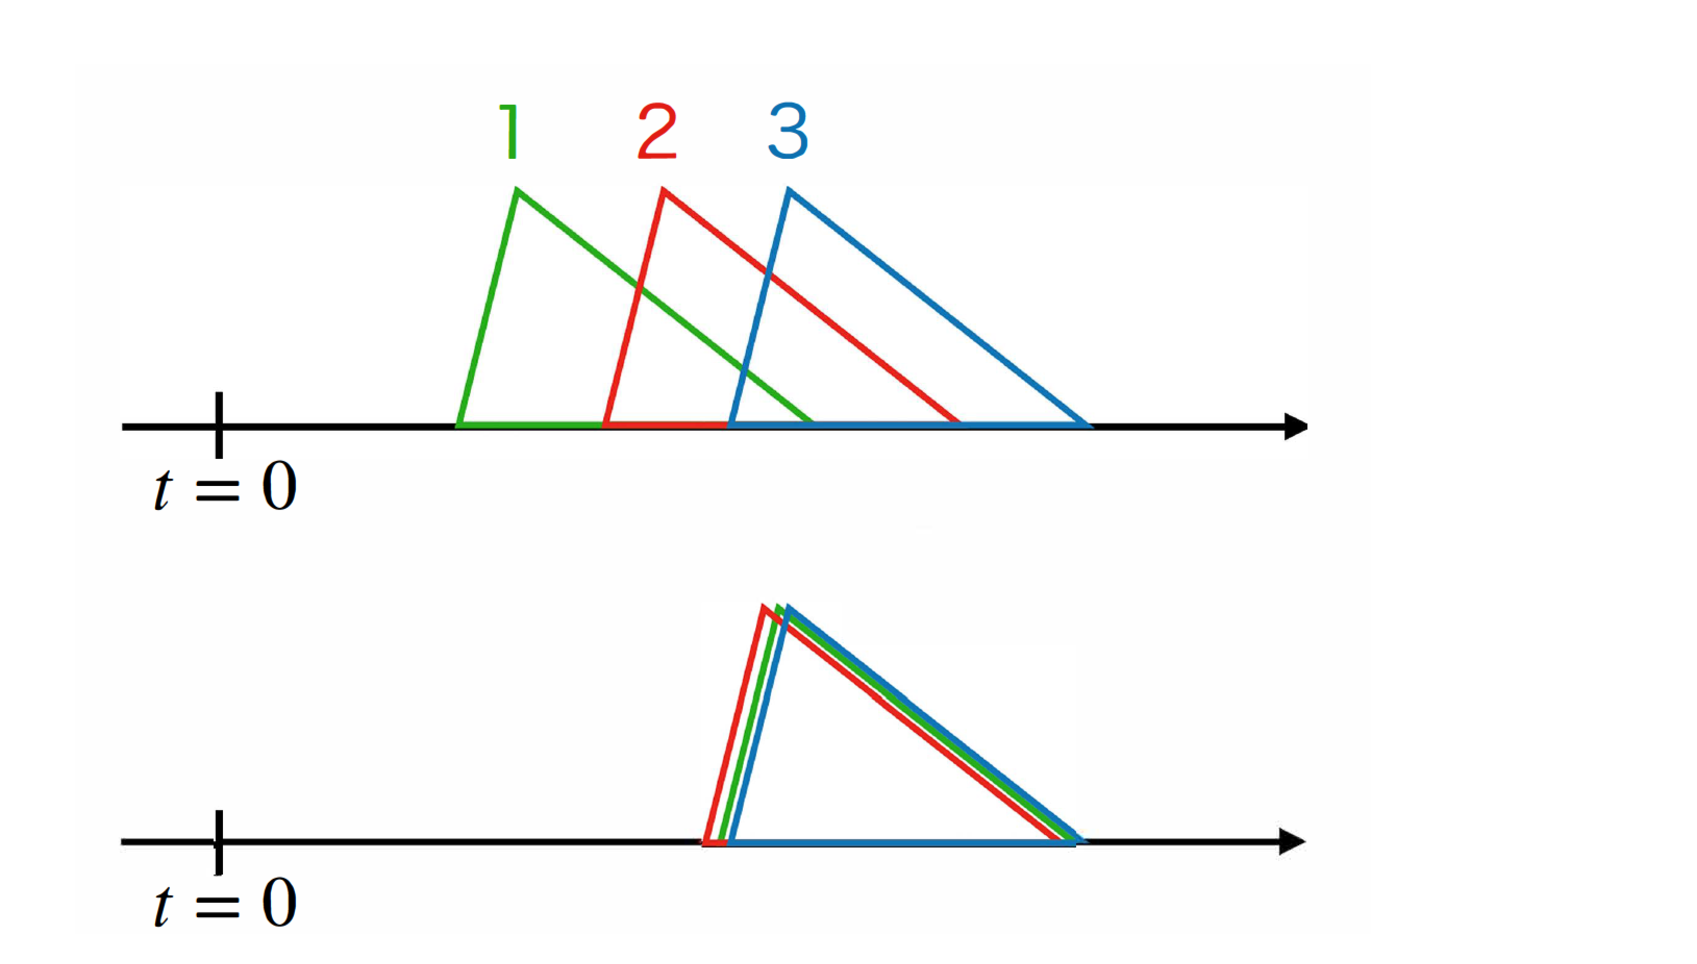
\includegraphics[width=0.8\textwidth,page=1]{img/slide/slide.pdf}
        \caption[信号タイミング調整の概念図]{信号タイミング調整の概念図~\cite{URL:09}。ケーブル~1,~2,~3~における入力タイミングの確率分布を示している。タイミング調整は一番遅く到達するケーブルに合わせて遅延するように行われている。遅延を調整できる最小単位は、PP~ASIC~の~Port-A,~Port-B~の単位。}
        \label{fig:delay}
\end{figure}

\begin{figure}[H]
        \centering   
        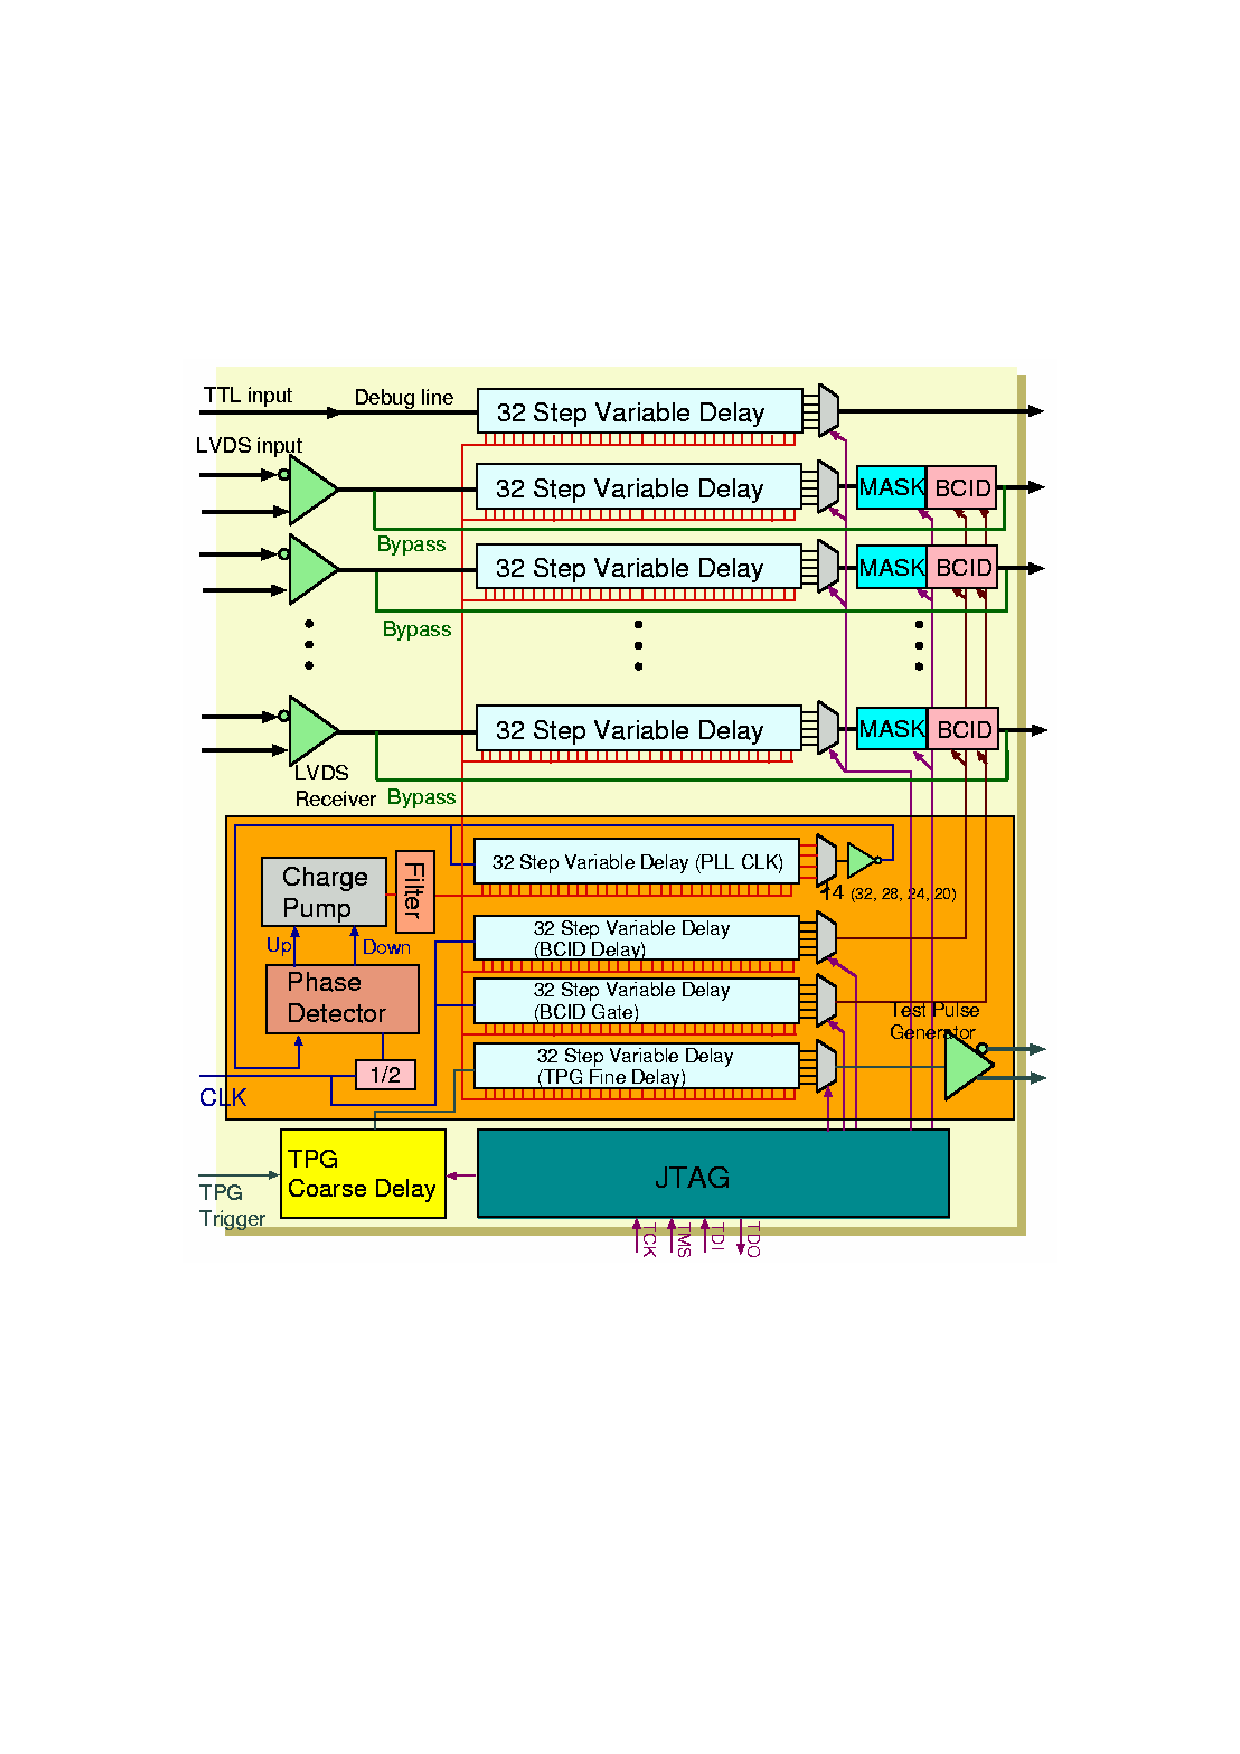
\includegraphics[width=0.8\textwidth,page=1]{img/pdf/PP.pdf}
        \caption[PP ASIC での信号処理の流れ]{PP ASIC での信号処理の流れ~\cite{URL:05}。入力信号に対して遅延がかけられ、Mask~および~BCID~が行われる。}
        \label{fig:PP}
\end{figure}

\subsubsection{バンチ交差識別}\label{subsubsec:bcid}
BCID~回路は~TGC~のヒット信号の立ち上がりを検出し、バンチ判定を行う。一つのインプットに対して、2~バンチのヒット情報を出すわけではない。TGC~ゲートはクロックの立ち上がりのタイミングと同期する。したがって同期したゲート幅内に~TGC~の生信号の立ち上がりが来るように幅を定義している。\figref{fig:clock}に信号の時間分布に対するクロック位相の調整方法についてを示す。

TGC~出力信号は内在的な時間分解能の影響で陽子衝突間隔~25~ns~より大きい。特に~strip~ではセンサーの長さとドリフト時間の影響が大きい(時間分解能:約~30~ns(wire)、約~40~ns(strip))。そのため信号の時間分布に対して、十分なゲート幅ならびにノイズ等の影響を鑑みて最小限のゲート幅を確保することが非常に重要である。\figref{fig:gate0}に例として信号の時間分布に対するゲート幅の調整方法についてを示した。図中の三角形は、1~事象の波形ではなく、バンチ交差を起点に~PP~で検出される信号の立ち上がり時間の確率分布関数を示していて、この分布の幅が内在的な時間分解能を表している。TGC~における~BCID~ゲート幅は可変(26-48~ns)で~PP~において決められたゲート幅が設定されている。\figref{fig:bcidgate}は可変なゲート幅を最小および最大に設定した場合のゲートの状態を示したものである。Run~2~におけるゲート幅の設定は\tbref{tb:BCIDGate}のようになっている。

以上の要領で設定された~BCID~回路によりバンチ交差識別を行う。バンチ判定を図式的に表現すると\figref{fig:bcid0}のように表すことができる。25~ns~おきの~LHC~クロックに対して、前のバンチ、基準バンチおよび次のバンチの~BCID~ゲートが設定されている状態である。そして\tbref{tb:BCIDGate}に示したようにゲート幅は、25~ns~よりも大きな幅がとられている。これは~BCID~ゲートに重なりを持たせることで不定性の削減を行うためである。したがって~TGC~におけるバンチ判定は、前のバンチ、前かつ基準バンチ、基準バンチ、基準かつ次のバンチ、次のバンチの~5~段階で行われる。光速のミューオンは信号の時間的揺らぎを考慮した上で基準バンチで判定されるように調整されている。

\begin{figure}[H]
        \centering   
        \includegraphics[width=0.8\textwidth,page=2]{img/slide/slide.pdf}
        \caption[クロック位相の調整]{クロック位相の調整~\cite{URL:09}。40~MHz~の~LHC~クロックの立ち上がりに対して、入力タイミングの確率分布の始まりを合わせるように位相を調整している。}
        \label{fig:clock}
\end{figure}
\begin{figure}[H]
        \centering   
        \includegraphics[width=0.8\textwidth,page=3]{img/slide/slide.pdf}
        \caption[BCID~ゲート幅の調整]{BCID ゲート幅の調整~\cite{URL:09}。入力タイミングの確率分布がすべて収まるように、BCID~ゲートの幅が調整されている。}
        \label{fig:gate0}
\end{figure}
\begin{figure}[H]
        \centering   
        \includegraphics[width=0.8\textwidth,page=4]{img/slide/slide.pdf}
        \caption[BCID~判定の概念図]{BCID~判定の概念図。LHC~クロックに対して、BCID~ゲートが設定されており、入力信号のタイミングにより、前のバンチ、前かつ基準バンチ、基準バンチ、基準かつ次のバンチ、次のバンチの~5~段階で判定が行われる。}
        \label{fig:bcid0}
\end{figure}

\begin{table}[tbp]
	\centering
	\begin{tabular}{c|l}\hline
	& \multicolumn{1}{c}{BCID Gate} \\ \hline
	BW wire & 29.32 ns(26 ns + 4 × 0.83 ns)\\
	BW strip & 40.94 ns(26 ns + 18 × 0.83 ns)\\
	SW wire & 33.47 ns(26 ns + 9 × 0.83 ns)\\
	SW strip & 45.09 ns(26 ns + 23 × 0.83 ns)\\
	\end{tabular}
	\caption{Run~2~における~BCID~ゲートの設定値}
	\label{tb:BCIDGate}
\end{table}

\begin{figure}[H]
		\begin{minipage}{0.49\hsize}
		\centering
        \includegraphics[width=0.9\textwidth,page=3]{img/pdf/PP.pdf}
        \subcaption{}
        \end{minipage}
        \begin{minipage}{0.49\hsize}
        \centering
        \includegraphics[width=0.9\textwidth,page=4]{img/pdf/PP.pdf}
        \subcaption{}
        \end{minipage}
        \caption[BCID ゲートの調整]{BCID~ゲートの調整~\cite{URL:05}。(a)~ステップが~0~(最小)の場合。(b)~ステップが~26~(最大)の場合。}
        \label{fig:bcidgate}
\end{figure}

\subsubsection{Slave~Board~ASIC}
Slave~Board~ASIC(SLB)は~TGC~出力信号のコインシデンス処理ならびに読み出し処理を行う役割を持ち、トリガー系とリードアウト系に区分される。以下では、リードアウト系に関する事項について説明する。

SLB~は~160~bits~の入力ポートを持ち、最大~160~チャンネルのヒットパターンが入力される。リードアウト系における~SLB~の役割は、受信した~160~bits~の情報を~L1A~を受け取るまで一時的にバッファにデータを保持しておくことである。
L1A~の信号を受信した後には、対応するデータに加えて前後~±1~バンチの情報も読み出し、それぞれ~Previous(前のバンチ)、Current(基準バンチ)、Next(次のバンチ)とタグ付けして~Star~Switch~に送信する。

\subsubsection{Star~Switch}
Star~Switch(SSW)は複数の~PSB~からの信号を~RDO~へと送信する役割を持つ。この際、転送するデータ量を減らすためにヒットがない情報は省く(zero-suppress)。SLB~からのデータは~Rx(レシーバー)に入力されデータの圧縮を行う。その後、Tx(トランスミッター)に送信され、フォーマットされる。フォーマットされたデータはシリアライズされ、RDO~に送られる。

\subsubsection{Read~Out~Driver}
Read~Out~Driver(RDO)は複数の~SSW~からシリアライズされた圧縮データを受信し、パラレルデータに戻しメモリーに一時格納する。このデータを、トリガー情報をもとに同一事象毎にまとめる。まとめられたデータは~S-LINK~という光信号で~ROS~に送信される。イベント同定のためには~TTC~からのトリガー情報が必要となるため、ROD~には受信のための~TTCrx~(TTC~Receiver~Chip)が搭載されている。

\subsection{トリガー系}
TGC~のトリガーは~BCID~された事象のセットを利用し、複数段のコインシデンス論理により、データサイズを減らしながら、コインシデンスロジックに用いる総数を増加させていくことで、最終的に~3~ステーションコインシデンスで~RoI~の決定および運動量の概算を行う。
\subsubsection{Slave~Board~ASIC}
BCID~され~LHC~クロックでサンプリングされたヒットは、L1~Buffer~に詰め込まれると同時に、SLB~のトリガーロジックに入力される。SLB~のトリガーロジックでは以下の演算を行っている。
\begin{itemize}
\item 2~層内、3~層内のコインシデンスおよびスタッガリングを用いた分解能の向上
\item M2,~M3~の間の~4~層でのコインシデンス
\end{itemize}
1~チップで各チェンバーの~32~チャンネルを処理する。チャンネルの種類の応じて~5~種類のコインシデンスマトリックス(wire~doublet,~strip~doublet,~wire~triplet,~strip~triplet,~EIFI)を切り替えて利用している。$\eta$~方向に見た場合、TGC~の~doublet~内及び~triplet~~内でスタッガリング構造(層ごとに~TGC~の位置が少しずれて配置されている)を持つため、コインシデンスによりデータ量を減らすのみでなく、位置分解能の向上にも起因する。
triplet~の~wire~SLB~トリガー回路では、3~層内でのコインシデンス処理を行う。3~層中~2~層のヒットを要求し、3~層の生信号を利用して~M1~に代表するヒットポイントを計算する。このロジックは~1~clock~サイクルで十分に終わることができるような設計となっている。ヒット情報の入力後、次のクロックの立ち上がりに演算結果が出力され~HPT~に送信される。複数のコインシデンス結果が見つかった場合は、代表するヒットを選び出すロジックの実装により~1~clock~で送信できるような設計になっている。同様に~strip~SLB~のトリガー回路は、M1~の~2~層中~1~層を要求するロジックで実装されている。
doublet~の~SLB~は、M2~と~M3~の~4~層を担当している。まず、M2~と~M3~の間で~2~層中~1~層のコインシデンス処理を行い、M2,~M3~で~4~層中~3~層のコインシデンスがとられる。

\subsubsection{High~PT~Board}
High~PT~Board(HPT)は~SLB~の出力を用いて、doublet(M2-M3),~triplet(M1)の間のコインシデンス処理を行う。SLB~のトリガー出力情報には以下が含まれている。
\begin{itemize}
\item M1~のヒット点の情報($R_1,~\phi_1$)
\item M3~のヒット点の情報($R_3,~\phi_3$)と、M2-M3~の差分($dR_{32},~d\phi_{32}$)
\end{itemize}
$R$~方向の~wire~コインシデンスと、$\phi$~方向の~strip~コインシデンスが別々に実行される。
SLB~と同様に、コインシデンスマトリックスを用いて計算は行われ、計算は~1~clock~サイクルで完了する。M1~と~M3~の間でコインシデンス処理を行い、$|dR_{13}|<=15$,~$|d\phi_{13}|<=7$~の条件をクリアした候補(トラックレット)が~Sector~Logic(SL)に送信される。
\subsubsection{Sector~Logic}
TGC~トリガーの最終段は~Sector~Logic~Board(SL)で、$R$(wire)と$\phi$(strip)の独立な~HPT~出力を統合して、$p_{\rm{T}}$~情報を概算し、RoI~と~$p_{\rm{T}}$~情報をパックして、MUCTPI~に送信する。HPT~の出力には、($R_{3},~dR_{13}$),($\phi_{3},~d\phi_{13}$)が含まれるため、$R_3,~\phi_3$~の情報をもとに、RoI~が決定され、$dR_{13},~d\phi_{13}$~の情報をもとに~$p_{\rm{T}}$~が概算される。$p_{\rm{T}}$~閾値に変換する過程は、高速処理のためあらかじめ変換の計算を対応表にした~Look~Up~Table~によって行われる。1~つのトリガーセクターから~1~バンチ~2~RoI~まで出力することができる。

\subsection{コントロール系}
デジタル電気回路の制御は、電子回路に組み込まれたレジスタ(メモリ)の読み書きによって行われている。レジスタに対する命令による電気回路の動作決定や、値を読み出すための命令による電気回路の状態のモニターなどの役割を持つ。

\subsection{トリガータイミングコントロール系}
ATLAS~実験では~40~MHz~という高頻度衝突かつ広範囲に設置された検出器による影響で、全体での事象の同期は容易ではない。同期のために大きな役割を担っているのが、TTC~システムである。各検出器では事象の情報を読み出すために~L1A~を受信する必要がある。なおかつ事象を正しく識別するためには~LHC~の衝突との同期を行わなければならない。そのため~BC~clock(Bunch~Crossing~signal)を各検出器に配布している。事象の認識のために読み出しが行われた情報に対しては~EVID~および~BCID~が付与される。

実験全体を通して以上の~ID~の一貫性を保つためには、システム全体を同期する基準となる信号が必要である。それらの信号を~BCR(Bunch~Counter~Reset)と~ECR(Event~Counter~Reset)と呼ぶ。TTC~信号を送信するのは、各検出器に設置されている~TTCvi(TTC~VME~interface)である。TTCvi~から送信された信号は光ファイバーを通して~TTCrx(TTC~Receiver~Chip)に送られる。TTCrx~ではタイミング調整のために~TTC~信号に対してクロック位相を~100~ps~の単位で調節でき、L1A~や~BCR,~ECR~の信号を~0~15~clock~の範囲で遅延することができる。

\section{TGC~システムにおけるタイミング調整}
本章では、TGC~エレクトロニクスにおける詳細な仕組みについて記した。本節では、エレクトロニクスを正しく動作させる上でのタイミング調整の重要性について説明する。

\subsection{タイミング調整の重要性}
ATLAS~の各エレクトロニクスでは~BCID~と~L1ID~が付加され、TTC~システムから配布された基準信号との同期を取ることで、システム全体での整合性を保つ。
TGC~システムは、TTC~が全測定器に~L1A~を発行するための重要な役割を担っている。TGC~において正しいバンチ交差識別が行われていなければ、検出器全体としての事象の同期に影響を及ぼす。どのバンチ衝突から生じた粒子なのかを正しく識別をするには、各検出器においてタイミングの同期を行わなければならない。したがって~TGC~検出器のタイミング調整はトリガーを行う上で非常に重要な役割を持つ。

\subsection{TGC~システムにおけるタイミングのばらつき}
TGC~システムにおいて正しく~BCID~を行うには、バンチ衝突に対応して~25~ns~毎に開く~BCID~ゲートに荷電粒子の信号を適切に収めることが必要である。
しかし、ミューオンが衝突点から~TGC~まで届くまでの時間(Time-of-Flight)には位置による差があり(約~24~-~64~ns)、さらに粒子の信号を伝搬するための各ケーブルの長さは、位置によって様々であるため、細かなタイミング調整を行わなければ、BCID~のゲート幅(26~-~48~ns)に収まらない。\figref{fig:tof}に~TGC~の位置によるミューオンの飛来時間の違いを示した。総読み出しチャンネル~32~万の~TGC~におけるタイミング調整を行うには、詳細かつ精密な見積もりが必要となる。またゲート幅に関して、単純に幅を大きくするだけでは、誤ったコインシデンスの増加などが懸念されるため、最小かつ最適なタイミングでゲートを設定することが必要である。

次章では、モンテカルロシミュレーションおよび~Run~2~実験データを用いて、TGC~検出器におけるタイミング調整の調査を行う。

\begin{figure}[H]
    \centering   
    \includegraphics[width=0.8\textwidth,page=8]{img/slide/slide.pdf}
    \caption{ミューオンの~TGC~各ステーションにおける飛来時間の一例}
    \label{fig:tof}
\end{figure}
